\chapter{Proposta}
Nos estudos realizados por Canfora e Hassan não foi analisado os efeitos da entropia nas métricas sociais e de processo. Além disso não há uma ferramenta que monitore a entropia e as métricas do projeto.

O objetivo é construir uma ferramenta que monitore o valor da entropia de mudança e sua relação com as métricas sociais, de autoria e de processos dos projetos. A ferramenta terá seis módulos que serão apresentados a seguir:

\begin{figure}[h]
	\captionsetup{justification=centering}
	\includegraphics[width=\linewidth]{fluxogramaTCC.png}
	\caption{Fluxograma do funcionamento da ferramenta}
	\label{figura:fluxogramaimagem}
\end{figure}

\section{Coleta de dados}
O módulo de coleta de dados é responsável pela extração de dados dos projetos do Github e Git. Os dados serão obtidos utilizando o GHTorrent, a ferramenta Change Metrics e Github API V3. 

\section{Cálculo das métricas}
O módulo de cálculo das métricas irá realizar o cálculo após a extração dos dados no módulo de coleta de dados. Nessa etapa o usuário deverá informar quais métricas ele deseja calcular e em qual período de tempo. Para utilizar a ferramenta Change Metrics será necessário realizar um clone do projeto da data em que o usuário informar.

\section{Cálculo da entropia}
Este módulo que realiza o cálculo da entropia de cada arquivo do projeto no período que o usuário informar. As outras métricas serão calculadas nesse mesmo período. 

\section{Relatório de análise}

\section{Visualização de dados}
Este módulo irá mostrar os resultados com gráficos bidimensionais e uma visualização utilizando o método Treemapping, exibindo uma hierarquia de dados utilizando retângulos aninhados. Será feito um gráfico para cada métrica selecionada no módulo de cálculo de métricas, onde o eixo x será o tempo e o eixo f(x) será o valor da métrica. O Treemapping será utilizado para visualizar o valor da entropia em cada arquivo do projeto.

\begin{figure}[h]
	\captionsetup{justification=raggedright}
	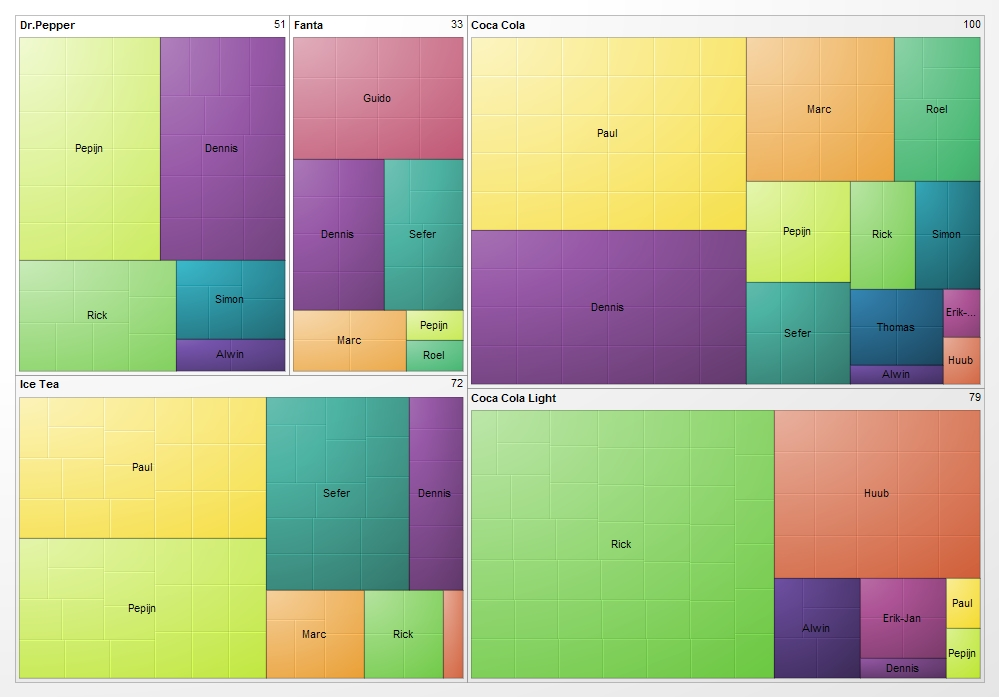
\includegraphics[scale=0.3]{treemap.jpg}
	\caption{Exemplo de visualização utilizando Treemapping.}
	\label{figura:visaometodo}
\end{figure}